\section{Objectives}
By the end of this lab work, students are expected to learn how to 

\begin{itemize}
    \item operate a DC power supply, a digital multimeter, and a breadboard (prototyping board) 
    \item measure resistance of a resistor using an ohmmeter and its color code
    \item measure voltages      
    \item measure currents
      
\end{itemize}

\section{Parts}
\label{sec:partsEx1}
The following parts are required to conduct this laboratory experiment. %
%
\begin{enumerate}           
\item Breadboard
\item Resistors: $100~[\ohm],$ $150~[\ohm],$ $220~[\ohm],$ $560~[\ohm],$  $1~[\kilo\ohm],$ $1.5~[\kilo\ohm],$ $2.2~[\kilo\ohm],$ $3.3~[\kilo\ohm],$ $10~[\kilo\ohm],$ and  $100~[\kilo\ohm].$
\end{enumerate}
  
\section{Laboratory Meters and Power Supply}
\label{sec:laboratoryMeters}

Electrical engineering fundamentals are verified using numerous laboratory instruments. Basic instruments (already installed in the laboratory workstation) that will be used throughout this course are listed below:
%
\begin{itemize}
\item Power supply
 
\item Digital multimeter
  
% \item Function generator
  
% \item Oscilloscope
\end{itemize}

These instruments are supposed to be mounted on each workstation in the
laboratory properly. In
this lab session, you will set up laboratory meters and power supply; and
measure voltage, current, and resistance using those meters. Laboratory safety
procedures should be reviewed before you start attempting to use any instrument
in this lab.


\subsection{Power Supply}
\label{sec:powerSupply}

Let us assume that the power supply installed in the laboratory workstation is shown in Figure~\ref{fig:agilentE3630A-PowerSupply}. The $35$-watt E3630A Agilent power supply provides three DC outputs: $0$ to $6 ~[\volt]$ with a maximum current of $2.5~[\ampere]$, a $0$ to $20~[\volt]$ output and a $0$ to $-20~[\volt]$ output with a maximum current of $0.5~[\ampere].$ This will typically act as a DC voltage source.%
%
\begin{figure}[h]
   \centering
   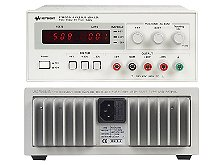
\includegraphics[width=0.5\textwidth]{figs/img/labs/agilentE3630A-PowerSupply.jpg}
   \caption{Agilent power supply (front and rear views).}
   \label{fig:agilentE3630A-PowerSupply}
\end{figure}
%

\subsection{Digital Multimeter}
\label{sec:digital-multimeter}

The digital multimeter installed in the laboratory workstation is shown in
Figure~\ref{fig:fluke45}. The Fluke 45 DMM is capable of measuring voltage,
current, and resistance. When measuring voltage and resistance, the red probe is
connected to the plug marked with a ``$\volt\ohm$'' and the black probe is
connected to the plug marked with a ``COM.'' The probes are then placed in
\emph{{\bf parallel}} with the desired circuit element to find the voltage or
resistance across it. When measuring the current, the red probe is connected to
the plug marked $10~\ampere$ first and then, if necessary, the
$100~\milli\ampere$~plug. The probes are then placed in \emph{{\bf series}} with
the element you want to find the current entering or exiting [\emph{show your
  connection to the instructor before turning on the circuit for operation}].


\begin{figure}[h]
    \centering
    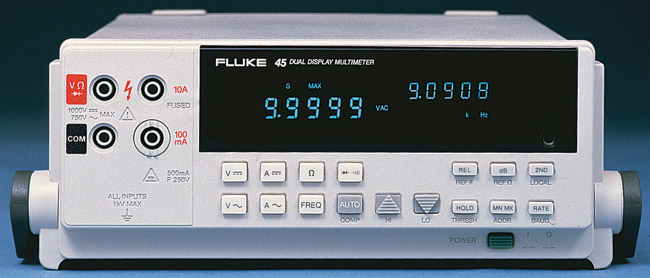
\includegraphics[width=0.5\textwidth]{figs/img/labs/fluke45.jpg}
    \caption{Fluke $45$ digital multimeter.}
    \label{fig:fluke45}
\end{figure}



% \subsection{Function Generator}
% \label{sec:functionGenerator}
% The function generator installed in the laboratory workstation is shown in Figure~\ref{fig:Agilent33210A-FunctionGenerator}. This instrument will output desired Voltage waveforms with a frequency range of 1Hz to 10MHz. It can produce ramp, triangle, pulse, sine and square waveform outputs as well as allow for AM, FM and PWM modulation.

% \begin{figure}[H]
%     \centering
%     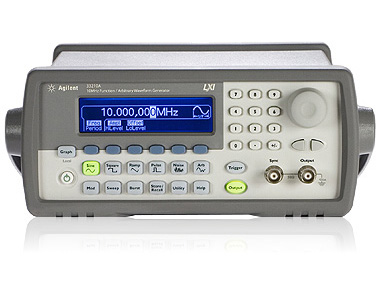
\includegraphics[width=0.5\textwidth]{figs/img/labs/Agilent33210A-FunctionGenerator.jpg}
%     \caption{Agilent Function Generator used in the Laboratory.}
%     \label{fig:Agilent33210A-FunctionGenerator}
% \end{figure}




\section{Breadboard}
\label{sec:breadboard}

A breadboard (also called ``protoboard'') is a platform on which a simple electrical/electronic circuit can be built and tested. It is widely used in academia for demonstrating simple electrical/computer engineering circuits. Throughout this course, you will be using a breadboard to demonstrate your lab tasks. 

Figure~\ref{fig:BB400-Solderless}  shows a typical breadboard used for laboratory tasks. It is recommended that you use the red (blue/black) horizontal row to connect the positive (negative) power supply lead. The connections among different holes/points are illustrated using the schematic diagram of a breadboard as shown in  Figure~\ref{fig:BB-Schematic}. Following Figure~\ref{fig:BB-Schematic}, the connections among holes/points in a breadboard are briefly described as follows. %
%
\begin{figure}
  \centering
  \subfigure[][]{
    \label{fig:BB400-Solderless}
    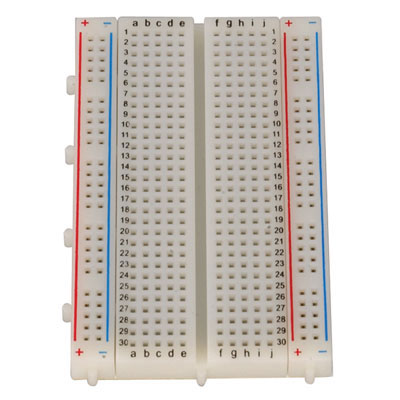
\includegraphics[width=0.45\textwidth]{figs/img/BB400-Solderless.jpg}
  }
  \subfigure[][]{
    \label{fig:BB-Schematic}
  \tikzset{
    open socket/.style = {
      circle,
      fill = black,
      inner sep = 1pt
    },
    filled socket/.style = {
      circle,
      fill = black,
      inner sep = 1pt
    }
  }
  \fcolorbox{yellow!20}{yellow!20}{
  \begin{tikzpicture}
%% draw breadboard sections
  \foreach \y [evaluate = \y as \line using int(abs(\y))] in {0, ..., -24}{

    % draw line numbers off to the left
    \node [text=gray] at (-3.7, 0.3*\y) {{\small \line}};
    \node [text=gray] at (3.7, 0.3*\y) {{\small \line}};

    % draw bus and breadboard grid sockets
    \foreach \lab/\x in {l-/-8, lg/-7, a/-5, b/-4, c/-3, d/-2, e/-1, f/1, g/2, h/3, i/4, j/5, rg/7, r+/8} {
      \coordinate [open socket] (\lab\line) at (0.4*\x, 0.3*\y);
    }

    % draw row connectivity for board proper
    \draw [lightgray, opacity = 0.4, very thick]
      (0.4*-5, 0.3*\y) -- (0.4*-1, 0.3*\y)
      (0.4*1, 0.3*\y)  -- (0.4* 5, 0.3*\y);

  }

  % label breadboard columns

  \foreach \lab/\x in {a/-5, b/-4, c/-3, d/-2, e/-1, f/1, g/2, h/3, i/4, j/5} {
    \node [above of = \lab0] {\lab};
  }

  % label buses

  \node [above of=l-0,rotate=90] {V$_{+}$};
  \node [above of=lg0,rotate=90] {GND$_{}$};
  \node [above of=rg0,rotate=90] {V$_{+}$};
  \node [above of=r+0,rotate=90] {GND$_{}$};

  % draw bus connection lines
  \begin{scope} [
      on background layer  % these paths should not interfere with anything else
    ]
    \draw [very thick, red,  opacity = 0.6] (l-0) -- (l-24);
    \draw [very thick, blue, opacity = 0.6] (lg0) -- (lg24);

    \draw [very thick, red, opacity = 0.6] (rg0) -- (rg24);
    \draw [very thick, blue,  opacity = 0.6] (r+0) -- (r+24);
  \end{scope}    
  \end{tikzpicture}
} % \fcolorbox
} 
  \caption{\subref{fig:BB400-Solderless} 400-point solderless breadboard (courtesy of \url{www.jameco.com})  and~\subref{fig:BB-Schematic} Schematic diagram of a breadboard showing connections among different points/holes.}
  \label{fig:breadboard}
\end{figure}

\begin{itemize}
\item Five holes of a vertical row are connected (shorted) internally, therefore, the voltage difference between any two holes in the same vertical row is ideally zero. 
\item The connections among vertical rows are open (disconnected), \textit{i.e.,} one vertical row is disconnected from the other vertical rows.
\item The holes in each of the horizontal rows (rows that are marked in red and blue) are connected (shorted) internally.
  However, holes in one horizontal row are disconnected (open) from that of
  other horizontal row(s). Some breadboards may have two horizontal rows in the
  same line broken in the middle. In that case, the holes in one horizontal row
  are disconnected from that of other horizontal row in the same line.
\end{itemize}


\section{Measurement of Basic Electrical Quantities}
\label{sec:measurement}


Throughout the laboratory work of this course, you will be using voltages in the range of $0~\volt$ to $24~\volt$ (low voltage) for the operation of electrical/electronic circuits.  The circuit in operation (as long as the power is supplied to the circuit) should remain \emph{untouched} for the sake of safety. As you already know, an electrical circuit requires a voltage source which is connected with a closed path for the current to flow. In most cases, you will be using a constant (DC) voltage that is supplied by a regulated power supply (see Figure~\ref{fig:agilentE3630A-PowerSupply}). The regulated power supply mounted on the laboratory workstation converts alternating current (AC) line power into a constant DC voltage.  

It is a good practice to measure the supply voltage (or the voltage of any node of the circuit you are analyzing) using a \emph{voltmeter}. The resistance of a resistor opposes the flow of current through a branch of a circuit. This quantity can be measured using an \emph{ohmmeter}. The current flowing through a branch of an electrical circuit can be measured using an \emph{ammeter}. All these three basic meters are integrated into a single meter called a \emph{digital multimeter} (explained previously), which is mounted on each workstation in the laboratory. 



\subsection{Measurement of Voltage and Current}
\label{sec:voltageCurrentMeasurement}

To measure the voltage across and the current through an electrical element (\textit{e.g.,} resistor), a power supply is to be connected with the element first. %
%
\begin{itemize}
\item When measuring voltage of a branch connecting between two nodes (points) in an electrical circuit, connect the voltmeter  in parallel with the branch (see Fig.~\ref{fig:DMMDiagram} where the DMM (voltmeter) is connected in parallel with a resistor).
%
\begin{figure}
  \centering
  \begin{circuitikz}[american]
    \draw[red] (0,0) to[short,*-] (0,4*\smgrid) to[short,-*]
    (2*\smgrid,4*\smgrid); \draw (2*\smgrid,4*\smgrid) to[V,l=Power
    supply,-*,fill=green!50] (8*\smgrid,4*\smgrid) --(10*\smgrid,4*\smgrid)
    to[short,-*] (10*\smgrid,0); \draw (0,0) to[R,l=Resistor] (10*\smgrid,0);
    \draw[->] (-\smgrid,2*\smgrid) node[left]{Red lead} -- (0,2*\smgrid);
    \draw[->] (11*\smgrid,3*\smgrid) node[right]{Black lead} --
    (10*\smgrid,3*\smgrid); \draw[red] (0,0) to[short,*-] (0,-4*\smgrid)
    to[short,-*] (2*\smgrid,-4*\smgrid); \draw (2*\smgrid,-4*\smgrid)
    to[voltmeter,v>=~,l=Voltmeter (DMM),-*,fill=yellow!50]
    (8*\smgrid,-4*\smgrid) --(10*\smgrid,-4*\smgrid) to[short,-*]
    (10*\smgrid,0);
  \end{circuitikz}
  % 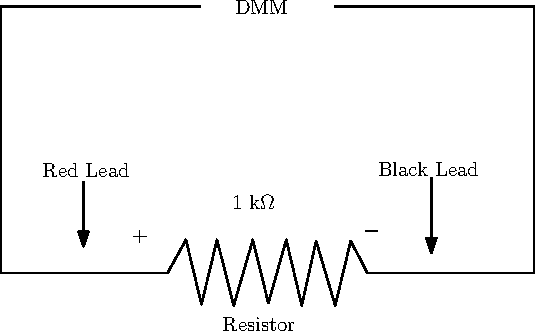
\includegraphics[width=0.6\textwidth]{figs/ipe/lab1/DMMDiagram}
    % \caption{DMM connection diagram in measuring resistance/voltage across a resistor.}  
    \caption{DMM connection diagram in measuring voltage across a resistor.}
    \label{fig:DMMDiagram}
\end{figure}
%
\item To measure current in a branch, connect the ammeter in series with the branch as shown in Figure~\ref{fig:DMMDiagramAmmeter}.  
%
\begin{figure}
  \centering
  \begin{circuitikz}[american]
    \draw[red] (0,0) to[short] (0,4*\smgrid) to[short,-*] (2*\smgrid,4*\smgrid);
    \draw (2*\smgrid,4*\smgrid) to[V,v>=Power supply,-*,fill=green!50]
    (8*\smgrid,4*\smgrid) --(15*\smgrid,4*\smgrid) to[short,-*] (15*\smgrid,0);
    \draw[red] (0,0) to[short,-*](2*\smgrid,0); \draw (2*\smgrid,0)
    to[ammeter,v>=~,l= Ammeter (DMM),-*,fill=yellow!50](8*\smgrid,0); \draw
    (8*\smgrid,0) to[R,l=Resistor] (15*\smgrid,0); \draw[->]
    (-\smgrid,2*\smgrid) node[left]{Red lead} -- (0,2*\smgrid); \draw[->]
    (16*\smgrid,3*\smgrid) node[right]{Black lead} -- (15*\smgrid,3*\smgrid);
  \end{circuitikz}  
    \caption{DMM connection diagram in measuring current through  a resistor.}
    \label{fig:DMMDiagramAmmeter}
\end{figure}
%
\end{itemize}

\subsection{Measurement of Resistance}
\label{sec:resistanceMeasurement}

When measuring  resistance of a branch connected between two nodes (points) in an electrical circuit, connect the  ohmmeter in parallel with the branch as shown in Figure~\ref{fig:DMMDiagramResistance}. %
%
\begin{figure}
  \centering
  \begin{circuitikz}[american]
    \draw[red]
    (0,0) to[short,*-] (0,4*\smgrid) to[short,-*] (2*\smgrid,4*\smgrid);
    \draw
    (2*\smgrid,4*\smgrid) to[ohmmeter,v>=Ohmmeter (DMM),-*,fill=yellow!50] (8*\smgrid,4*\smgrid) --(10*\smgrid,4*\smgrid) to[short,-*] (10*\smgrid,0);
    \draw
    (0,0) to[R=$1$<{[}\kilo\ohm{]}>,l=Resistor] (10*\smgrid,0);
    \draw[->]
    (-\smgrid,2*\smgrid) node[left]{Red lead} -- (0,2*\smgrid);
    \draw[->]
    (11*\smgrid,3*\smgrid) node[right]{Black lead} -- (10*\smgrid,3*\smgrid);
  \end{circuitikz}
  % 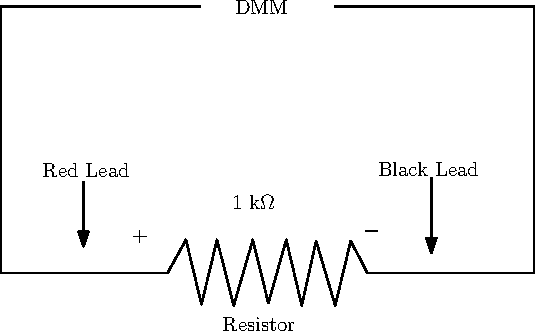
\includegraphics[width=0.6\textwidth]{figs/ipe/lab1/DMMDiagram}
    % \caption{DMM connection diagram in measuring resistance/voltage across a resistor.}  
    \caption{DMM connection diagram in measuring resistance of a resistor.}
    \label{fig:DMMDiagramResistance}
\end{figure}
%
The resistance of a resistor can be fixed or variable. The value of the
resistance of a fixed resistor can be determined by a four-band color code
displayed on the resistor (see Fig.~\ref{fig:resistanceColorCode4-Band}). Each
color corresponds to a number as shown in Table~\ref{tab:resistanceColorCode}.
The resistance value of a resistor is determined by the first three color bands.
For example, if the first, second, and third color bands are \emph{Red},
\emph{Black}, and \emph{Orange}, respectively, then the value of the resistance
is $20\times 10^3~[\ohm].$ Note that the fourth color-band indicates the tolerance
of the resistor, which is $\pm 5\%,$ $\pm 10\%,$ and $\pm 20\%$ for \emph{Gold},
\emph{Silver}, and \emph{No band}, respectively. Therefore, taking into account
the fourth band (silver), the resistance value of our example is $20\times 10^3~[\ohm] \pm
10\%.$ %
%
%
\begin{figure}
    \centering
    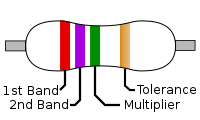
\includegraphics[scale=0.5]{figs/img/labs/resistanceColorCode4-Band}
    \caption{Color code of a 4-band  resistor (source: \url{https://www.wikipedia.org/}).}
    \label{fig:resistanceColorCode4-Band}
\end{figure}
%



\begin{table}
    \caption{Color code in determining the resistance.}
    \centering
    \begin{tabular}{|l||c|c|c|c|c|c|c|c|c|c|}
    \toprule
      \cellcolor{yellow!30}{\bf Color} & Black & Brown & Red & Orange & Yellow & Green & Blue & Violet & Gray & White\\
      \hline
      \cellcolor{yellow!30}{\bf Digit} & 0 & 1 & 2 & 3 & 4 & 5 & 6 & 7 & 8 & 9\\
    \bottomrule         
    \end{tabular}
    \label{tab:resistanceColorCode}        
\end{table}


\begin{mdframed}[roundcorner=5pt,backgroundcolor=yellow!5]
  {\bf Don't forget to mention  the unit of every measurement.}
\end{mdframed}

 
\section{Laboratory Work}
\begin{enumerate}

\item  Adjust the Agilent power supply to provide a $10~[\volt]$ output and measure it with a digital multimeter.  Record the meter reading \underline{\hspace{2.0 cm}}. 
  
\item Supply $10~[\volt]$ from the Agilent power supply to the power supply
  rails (red and blue/black horizontal rows) of the breadboard (labeled with
  ``Horizontal row'' in Figure~\ref{fig:jameco25-Breadboard}). The breadboard
  ground (the row that is marked in black or blue) is to be connected with the
  power supply ground. %
  %
\begin{figure}
    \centering
    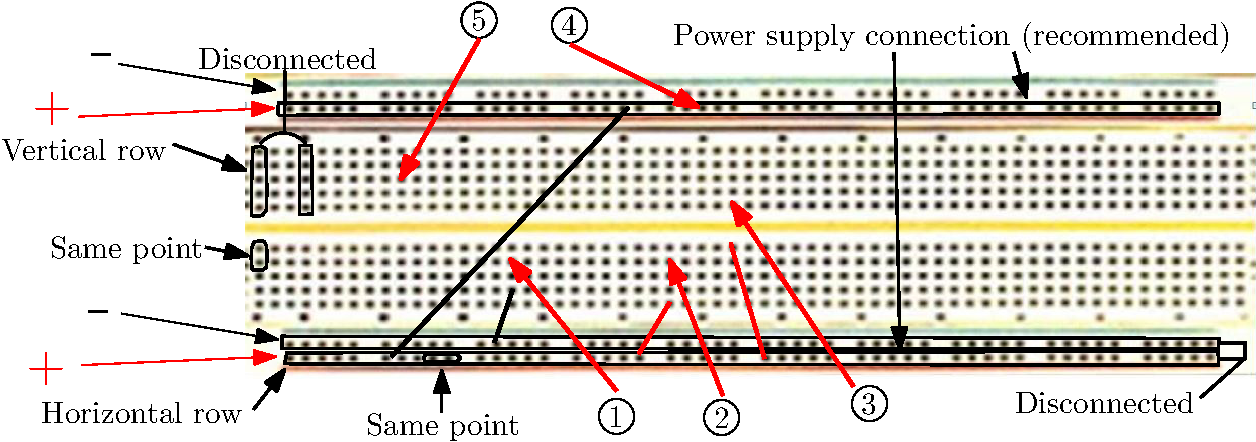
\includegraphics[width=0.8\textwidth]{figs/ipe/lab1/breadboardLayout}
    \caption{A breadboard (adapted from Jameco's 1660-Point solderless breadboard) showing connections among holes.}
    \label{fig:jameco25-Breadboard}
\end{figure}  
%
Connect holes with wires (connections are shown with straight lines in
Figure~\ref{fig:jameco25-Breadboard}). Measure voltages at five points (see the
point marked with \raisebox{.5pt}{\textcircled{\raisebox{-.9pt} {1}}},
\raisebox{.5pt}{\textcircled{\raisebox{-.9pt} {2}}},
\raisebox{.5pt}{\textcircled{\raisebox{-.9pt} {3}}},
\raisebox{.5pt}{\textcircled{\raisebox{-.9pt} {4}}}, and
\raisebox{.5pt}{\textcircled{\raisebox{-.9pt} {5}}} in
Figure~\ref{fig:jameco25-Breadboard}) with respect to the ground (holes in the
horizontal rows marked
in black/blue) of the
breadboard\footnote{Use a wire to connect one of the holes in horizontal
  black/blue line with the power supply ground.}. Justify illustrations as follows: %
%
\begin{itemize}
\item Voltmeter reading between point
  \raisebox{.5pt}{\textcircled{\raisebox{-.9pt} {1}}} and ground is
  \underline{\hspace{2.0 cm}}~[\volt] because
  \ul{~~~~~~~ ~~~~~~~~~ ~~~~~~~~ ~~~~~~~~~ ~~~~~ ~~~~~~~~~ ~~~~~~~ ~~~~~~
    ~~~~~~~ ~~~~~~~ ~~~~~~~~ ~~~~~~}.  
\item Voltmeter reading between point
  \raisebox{.5pt}{\textcircled{\raisebox{-.9pt} {2}}} and ground is
  \underline{\hspace{2.0 cm}}~[\volt] because
  \ul{~~~~~~~ ~~~~~~~~~ ~~~~~~~~ ~~~~~~~~~ ~~~~~ ~~~~~~~~~ ~~~~~~~ ~~~~~~
    ~~~~~~~ ~~~~~~~ ~~~~~~~~ ~~~~~~}.  
\item Voltmeter reading between point
  \raisebox{.5pt}{\textcircled{\raisebox{-.9pt} {3}}} and ground is
  \underline{\hspace{2.0 cm}}~[\volt] because
  \ul{~~~~~~~ ~~~~~~~~~ ~~~~~~~~ ~~~~~~~~~ ~~~~~ ~~~~~~~~~ ~~~~~~~ ~~~~~~
    ~~~~~~~ ~~~~~~~ ~~~~~~~~ ~~~~~~}.  
\item Voltmeter reading between point
  \raisebox{.5pt}{\textcircled{\raisebox{-.9pt} {4}}} and ground is
  \underline{\hspace{2.0 cm}}~[\volt] because
  \ul{~~~~~~~ ~~~~~~~~~ ~~~~~~~~ ~~~~~~~~~ ~~~~~ ~~~~~~~~~ ~~~~~~~ ~~~~~~
    ~~~~~~~ ~~~~~~~ ~~~~~~~~ ~~~~~~}.  
\item Voltmeter reading between point
  \raisebox{.5pt}{\textcircled{\raisebox{-.9pt} {5}}} and ground is
  \underline{\hspace{2.0 cm}}~[\volt] because
  \ul{~~~~~~~ ~~~~~~~~~ ~~~~~~~~ ~~~~~~~~~ ~~~~~ ~~~~~~~~~ ~~~~~~~ ~~~~~~
    ~~~~~~~ ~~~~~~~ ~~~~~~~~ ~~~~~~}.  
\end{itemize}

  
\item Construct the circuit shown in Figure~\ref{fig:DMMDiagramAmmeter} with $10~[\volt]$ power supply. Record the current flowing through the  $1~[\kilo\ohm]$ resistor. 
  
\item Obtain ten color coded resistors from the resistance tray in the
  laboratory's cabinet, measure their resistances, and compute the percentage
  $(\%)$ difference between the color-coded (ideal) and measured (actual) resistance values for
  all ten resistors using
 %
 \begin{align}
     \%~\text{difference} = \frac{\big|R_{\text{color-code}} - R_{\text{measured}}\big|}{R_{\text{color-code}}}\times 100\%,
     \label{eq:resistanceMeasurementError}
 \end{align}
 %
 where  $R_{\text{color-code}}$ and $R_{\text{measured}}$ are the color-coded
 (ideal) and measured (actual) resistance values, respectively. Then, complete the table below.
% pursue
  \begin{center}
    \begin{tabular}{c|c|c|c}
      \toprule
      Resistor \#& Ideal (color-coded)& Meter reading  (measured) & \%~\text{difference} using Equation~\eqref{eq:resistanceMeasurementError}\\
      \toprule
      1 & $100~[\ohm]$ & \underline{\hspace{2.0 cm}} & \underline{\hspace{2.0 cm}}\\
      2 & $150~[\ohm]$ & \underline{\hspace{2.0 cm}} & \underline{\hspace{2.0 cm}}\\
      3 & $220~[\ohm]$ & \underline{\hspace{2.0 cm}} & \underline{\hspace{2.0 cm}}\\
      4 & $560~[\ohm]$ & \underline{\hspace{2.0 cm}} & \underline{\hspace{2.0 cm}}\\
      5 & $1~[\kilo\ohm]$ & \underline{\hspace{2.0 cm}} & \underline{\hspace{2.0 cm}}\\
      6 & $1.5~[\kilo\ohm]$ & \underline{\hspace{2.0 cm}} & \underline{\hspace{2.0 cm}}\\
      7 & $2.2~[\kilo\ohm]$ & \underline{\hspace{2.0 cm}} & \underline{\hspace{2.0 cm}}\\
      8 & $3.3~[\kilo\ohm]$ & \underline{\hspace{2.0 cm}} & \underline{\hspace{2.0 cm}}\\
      9 & $10~[\kilo\ohm]$ & \underline{\hspace{2.0 cm}} & \underline{\hspace{2.0 cm}}\\
      10 & $100~[\kilo\ohm]$ & \underline{\hspace{2.0 cm}} & \underline{\hspace{2.0 cm}}\\
      \bottomrule
    \end{tabular}    
  \end{center}

\end{enumerate}

%%% Local Variables:
%%% mode: latex
%%% TeX-master: "../../labBookMechatronics-V2"
%%% End:
